%%
%% Author: K.Ooe
%% 2019/06/29
%%

% Preamble
\documentclass[11pt]{article}

% Packages
\usepackage{amsmath}

% Document
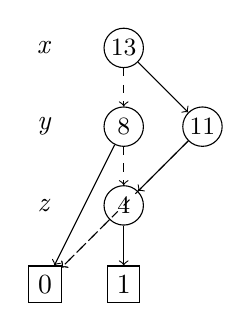
\begin{tikzpicture}[node distance=1cm]
    \tikzstyle{BDDnode}=[circle,draw=black,inner sep=0pt,minimum size=5mm]
    \node[] (vx) {$\mathit{x}$};
    \node[xshift=0cm, BDDnode, right of=vx] (n13) {\small $13$};

    \node[below of=vx] (vy) {$\mathit{y}$};
    \node[xshift=0cm, BDDnode, right of=vy] (n8) {\small $8$};
    \node[xshift=0cm, BDDnode, right of=n8] (n11) {\small $11$};

    \node[below of=vy] (vz) {$\mathit{z}$};
    \node[xshift=0cm, BDDnode, right of=vz] (n4) {\small $4$};


    % terminals
    \node[draw=black, style=rectangle, below of=vz, xshift=1cm] (n1) {$1$};
    \node[draw=black, style=rectangle, left of=n1] (n0) {$0$};

    % edges

    \draw[->,dashed] (n4) -> (n0);
    \draw[->] (n4) -> (n1);
    \draw[->,dashed] (n8) -> (n4);
    \draw[->] (n8) -> (n0);
    \draw[->,dashed] (n11) -> (n0);
    \draw[->] (n11) -> (n4);
    \draw[->,dashed] (n13) -> (n8);
    \draw[->] (n13) -> (n11);

\end{tikzpicture}